\documentclass[11pt,letterpaper]{article}

\newenvironment{proof}{\noindent{\bf Proof:}}{\qed\bigskip}

\newtheorem{theorem}{Theorem}
\newtheorem{corollary}{Corollary}
\newtheorem{lemma}{Lemma} 
\newtheorem{claim}{Claim}
\newtheorem{fact}{Fact}
\newtheorem{definition}{Definition}
\newtheorem{assumption}{Assumption}
\newtheorem{observation}{Observation}
\newtheorem{example}{Example}
\newcommand{\qed}{\rule{7pt}{7pt}}

\newcommand{\solution}[4]{
\thispagestyle{plain} 
\newpage
\setcounter{page}{1}
\noindent
\begin{center}
\framebox{ \vbox{
\vspace{4mm}
\vspace{0.2in} 
{\centering \large\mbox{#3}}\\
\vspace{0.1in}
{#1 \hfill {Date: #2}}
}}
\end{center}
\markright{#1}
}

\newenvironment{algorithm}
{\begin{center}
\begin{tabular}{|l|}
\hline
\begin{minipage}{1in}
\begin{tabbing}
\quad\=\qquad\=\qquad\=\qquad\=\qquad\=\qquad\=\qquad\=\kill}
{\end{tabbing}
\end{minipage} \\
\hline
\end{tabular}
\end{center}}

\def\Comment#1{\textsf{\textsl{$\langle\!\langle$#1\/$\rangle\!\rangle$}}}



\usepackage{graphicx, amssymb, amsmath, listings, float, mathtools}
\usepackage{color, url}
\lstset{language = Python}
\lstset{breaklines}
\lstset{extendedchars=false}
 
\definecolor{codegreen}{rgb}{0,0.6,0}
\definecolor{codegray}{rgb}{0.5,0.5,0.5}
\definecolor{codepurple}{rgb}{0.58,0,0.82}
\definecolor{backcolour}{rgb}{0.95,0.95,0.92}
 
\lstdefinestyle{mystyle}{
    backgroundcolor=\color{backcolour},   
    commentstyle=\color{codegreen},
    keywordstyle=\color{magenta},
    numberstyle=\tiny\color{codegray},
    stringstyle=\color{codepurple},
    basicstyle=\footnotesize,
    breakatwhitespace=false,         
    breaklines=true,                 
    captionpos=b,                    
    keepspaces=true,                 
    numbers=left,                    
    numbersep=5pt,                  
    showspaces=false,                
    showstringspaces=false,
    showtabs=false,                  
    tabsize=2
}
 
\lstset{style=mystyle}

\oddsidemargin 0in
\evensidemargin 0in
\textwidth 6.5in
\topmargin -0.6in
\textheight 9.0in

\begin{document}

\solution{\large Jifu Zhao}{\large 09/29/2016}{\bf \Large IE 529 \hspace{0.5cm} 
		Fall 2016 \hspace{0.5cm} Assignment 2}

\section{\large PCA}

Following the procedures of PCA, the mean value is:
$$\vec{m} = [1.87275, \  1.48783, \  1.87275]$$

And the variance is:
$$variance = [2.38297, \  0.234668, \  2.54 \times 10^{-16}]$$

And the corresponding eigenvector is: 
$$eig1 = [-0.6694 \ -0.3220 \  -0.6694]^T$$
$$eig2 = [0.2277 \  -0.9467 \  0.2277]^T$$
$$eig3 = [-0.7071 \  -1.4140 \times 10^{-15} \  0.7071]^T$$

The de-biased dataset and corresponding eigenvectors are plotted in Figure \ref{fig:3d}.

\begin{figure}[H]
\centering
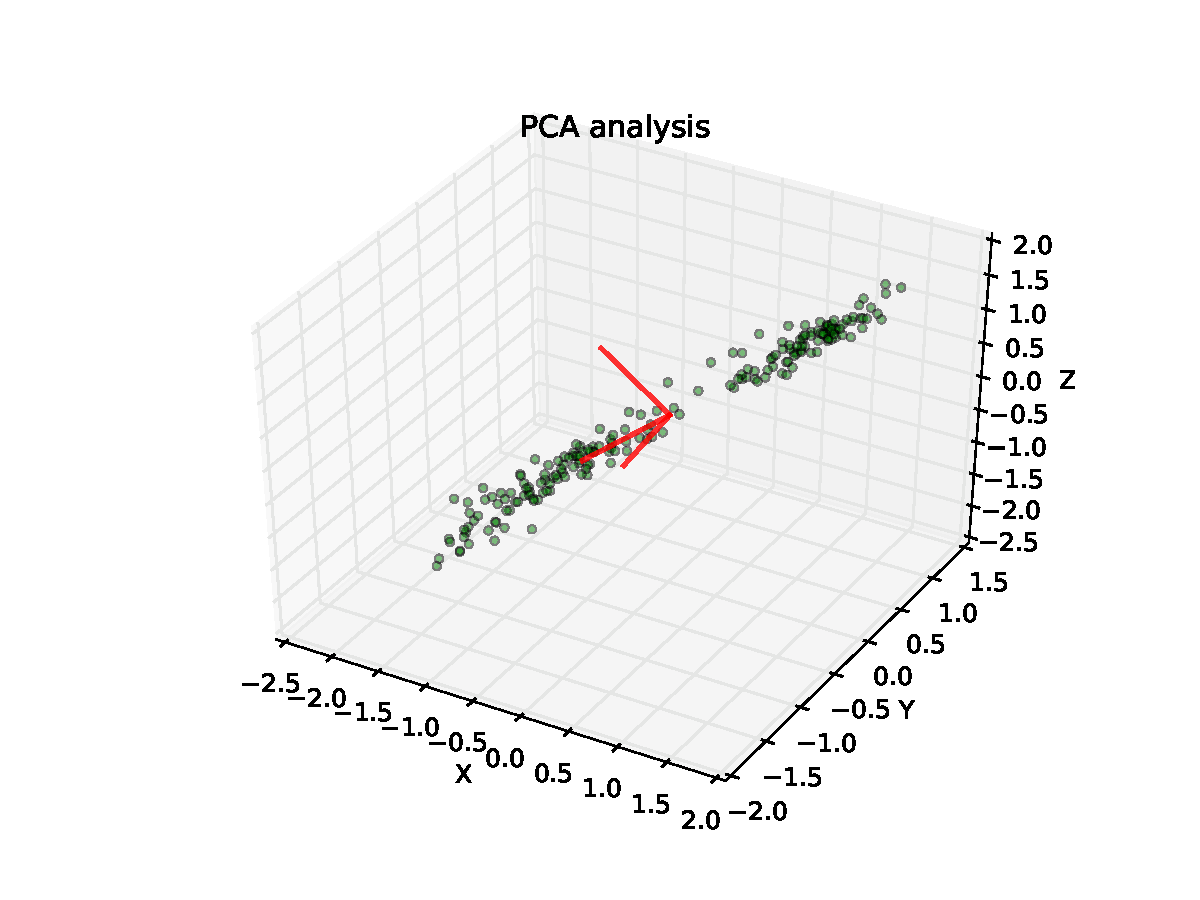
\includegraphics[width=0.9\textwidth]{./figures/3d.pdf}
\caption{\label{fig:3d} PCA eigenvector and scatter plot}
\end{figure}


The original dataset can be projected onto the first two principal components, the result is shown in Figure \ref{fig:projection}.
\begin{figure}[H]
\centering
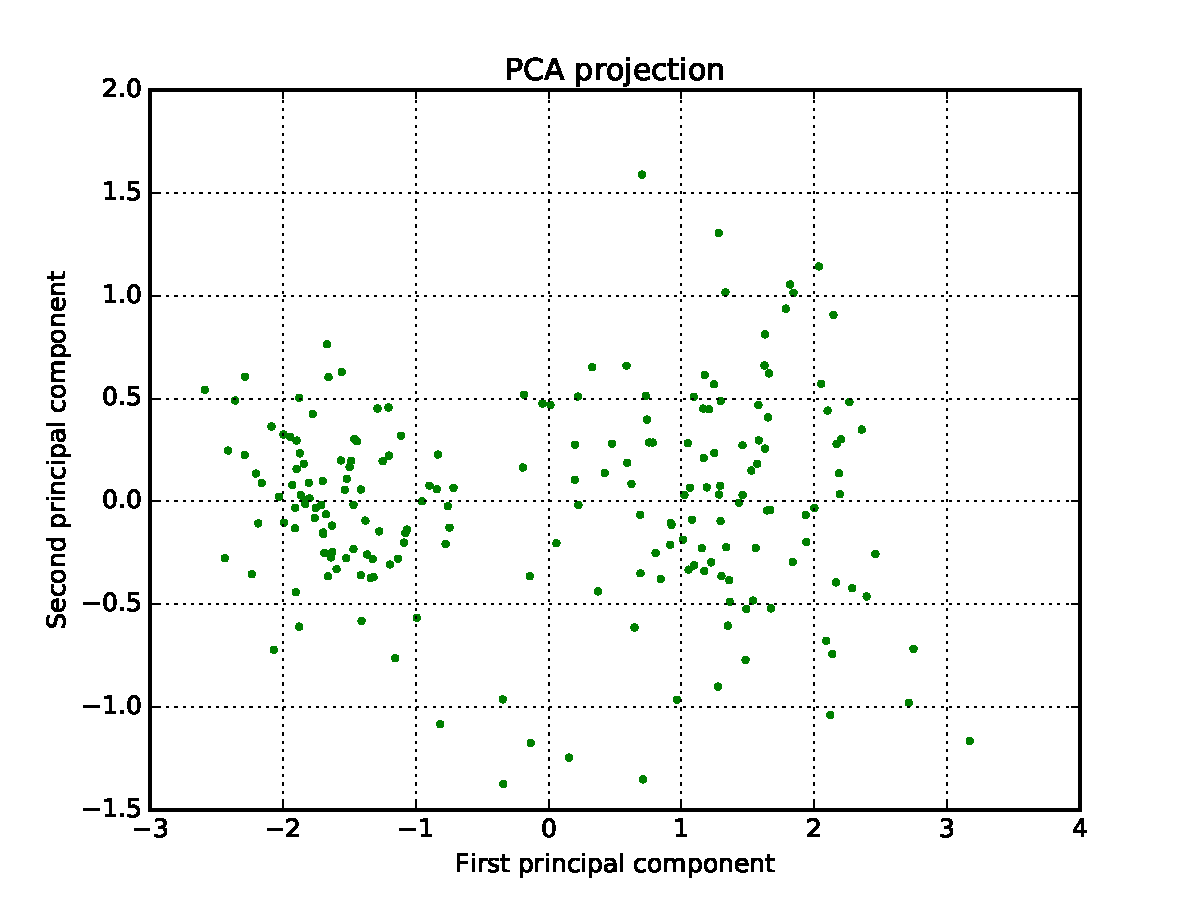
\includegraphics[width=0.9\textwidth]{./figures/projection.pdf}
\caption{\label{fig:projection} PCA Projection}
\end{figure}


\section{\large Discussion}

Currently the PCA is conducted through $$[U, S, V] = SVD(A * A^T)$$

In fact this process can be simplified to: $$[U', S', V'] = SVD(A)$$

Then, we can get that: 
$$U = U'$$
$$S = {S'} ^ 2$$

In this way, this process can be directly performed on the original data, rather than the new data.


The Python code is attached.

\newpage
\begin{lstlisting}
#!/usr/bin/env python3
# -*- coding: utf-8 -*-
"""
__author__      = "Jifu Zhao"
__email__       = "jzhao59@illinois.edu"
__date__        = "09/29/2016"
"""

import warnings
warnings.simplefilter('ignore')
import copy
import numpy as np
import pandas as pd
import matplotlib.pyplot as plt
from mpl_toolkits.mplot3d import Axes3D

def pca(data):
    """ function to perform PCA """
    data = copy.deepcopy(data)
    n, m = data.shape
    mean = np.mean(data, axis=0)
    data -= mean
    covariance = np.dot(data.T, data) / (n - 1)
    U, S, V = np.linalg.svd(covariance)
    return S, mean, U


def main():
    # PCA analysis
    data = pd.read_csv('./PCAdata.csv', header=None).values.T
    variance, mean, component = pca(data)
    project = np.dot(data - mean, component)
    data = data - mean

    print('Mean:\t', mean)
    print('Variance:\t', variance)
    print('Eigenvector 1\t', component[:, 0])
    print('Eigenvector 2\t', component[:, 1])
    print('Eigenvector 3\t', component[:, 2])

    # 3D plot
    fig = plt.figure()
    ax = fig.add_subplot(111, projection='3d')
    ax.plot(data[:, 0], data[:, 1], data[:, 2], 'o', markersize=4, color='green', alpha=0.5)
    for i in range(3):
        ax.plot([0, component[0, i]], [0, component[1, i]], [0, component[2, i]],
                color='red', alpha=0.8, lw=2)
    ax.set_xlabel('X')
    ax.set_ylabel('Y')
    ax.set_zlabel('Z')
    ax.set_title('PCA analysis')
    ax.view_init(40)
    fig.savefig('./result/3d.pdf')
    plt.show()

    # PCA projection
    fig, ax = plt.subplots()
    ax.plot(project[:, 0], project[:, 1], 'g.')
    ax.set_title('PCA projection')
    ax.set_xlabel('First principal component')
    ax.set_ylabel('Second principal component')
    ax.grid('on')
    fig.savefig('./result/projection.pdf')
    plt.show()


if __name__ == '__main__':
    main()
\end{lstlisting}

\clearpage

%\bibliographystyle{plain}
%\bibliographystyle{unsrt}
%\bibliography{reference.bib}

\end{document}

